\section{Route planning}
In order to be able to suggest routes to motorists, the system must find the best route available given at a given time and day of the week. One could define several quality measures of a good route, but in this case we consider the best route in terms of time, that is, the shortest travel time. The process is known as finding shortest paths in a directed weighted graph, and existing algorithms solve this problem well. In this section we discuss the methods used for finding such shortest paths.

\subsection{A* Heuristic Search}\label{sec:pathfinding}
We use the heuristic search algorithm A* since it is a widely used approach for finding shortest path routes in graphs and can be improved by further preprocessing of the graph as discussed in Chapter \ref{ch:future-work}.
We design the heuristic as an underestimate of the real travel time from a start node to target node, by letting the heuristic be the travel time of traveling the eucledian distance from the start node to the target node when traveling with the average speed of observations. 

Let $h(n)$ be the heuristic function:
\begin{align*}
h(v) = &\frac{avg(s_1,…,s_n)}{dist(u,v)} \qquad u,v \in E
\end{align*}
where $s_1,...,s_n$ are speeds of observations.
that computes an underestimate of the travel time from $u$ to $v$ to ensure the graph search proceeds in the correct direction in the graph.

At every expansion of a node, the weights of the frontier is computed by the respective weight functions for the given time, to determine the best next step in the path. The idea is illustrated in Figure \ref{fig:timed-graph} 
\begin{figure}[h]
\centering
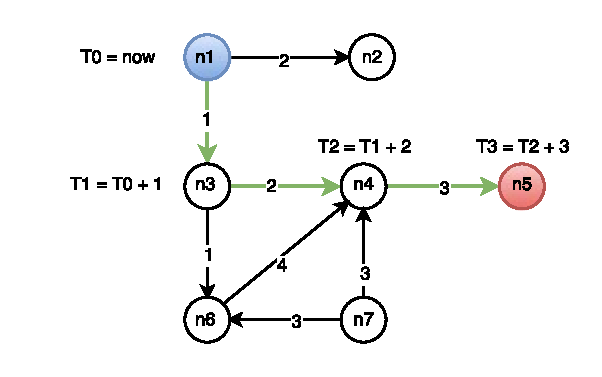
\includegraphics[width=\linewidth]{figures/timed-graph}
\caption{Relative times in path-finding - Numbers on edges are costs in time. Relative time is indicated next to nodes. The green arrows indicate the shortest path found. Each time is used as argument to the weight function for a segment.}
\label{fig:timed-graph}
\end{figure}

Whenever a road segment edge is chosen, the next node is expanded to get the available edges and their weght functions. The previous weight is added to the time, to make sure the next weight function is correctly selected. 
%An A* is used to finding a path through the graph. There are other versions of a A* search that are faster then a normal A*, but these do not work with the weight function that are being used. The time complexity of this search is $O(b^n)$ where $b$ is the branching factor and $n$ is the number of nodes in the graph.

%The function is given a start and a goal node, the A* utilise the physical destined between these point as a heuristic to make sure the path it takes goes in the right direction. Then it finds the time and ask the database for the cost of the segments it can travel from the node it's at. 

%The reason for using this algorithm over other graph search is that the the time for finding a path is $O(b^{(n/2)})$ where a normal Dijkstra’s takes $O(b^{n})$, where $b$ is the branching factor and $n$ is the number of nodes in the direct graph. Bi-directional also have the benefit of working well when running in paralleled.


% How do we use it?
%By using bi-directional search there is one problem that needs to be address, this is will the search meet op before the whole graph is search. There are more then one way of solving this problem, in this project A* have been chosen for solving this problem. The A* makes sure that the search from the start node wakes a path towards the end node and the other way around for the search that starts from end node.

%By implementing the bi-directional search this way, the worst case running time becomes $O(b^{n})$. The reason for this is that each search is going towards the other search's start node and not it's frontier. The search will stop if one of the two searches hits a node that the other search have visited.

\subsection{Weight function}\label{sec:weight-function}
The weight of road segments is the travel time required to travel along a road segment at a specific time and day of the week. With the regression model for predicting speed on a road segment from time and day of the week, we can compute a prediction for the travel time. 

Let
\begin{align}
weight: E \times T \times W \rightarrow \mathbb{R_+}
\end{align}
be the \emph{weight function} that maps an edge $e$, timestamp $t$, and day of the week $w$, to a positive, real-valued travel time.

The weight function works, by calculating the $speed$ function described in Equation \ref{eq:speed-piecewise} and dividing the predicted speed by the length of the given road segment. That is, given $e \in E$, $t \in T$, $w \in W$:
\begin{align}
weight(e,t,w) = \frac{speed(e,t,w)}{len(e)}
\end{align}
where:
\begin{align}
len:E \rightarrow \mathbb{R_+}
\end{align}
is a length function, that maps edges to their length.
Using the travel time as the weight for edges are more interesting in terms of time savings, than using directly the distance of the road.